


\chapter{构建三维人体姿态数据库}
由于人体姿态估计算法大部分为监督学习,因此研究者制作了很多用于训练和测试的数据库,这些数据库有些是从互联网、电影中获得的图片,并人工标记出骨架作为ground-truth,有些是通过标记点或传感器等手段在拍摄影像的同时记录人体姿态的ground-truth。表\ref{tab:benchmark}整理了目前常用的人体数据库,本文采用了HumanEva-I~\cite{sigal2006humaneva}数据库,将在\ref{sec:HumanEva}节介绍。

\begin{table}[htbp]
  \centering
  \renewcommand{\arraystretch}{1.5}
  \begin{minipage}[t]{\linewidth} % 如果想在表格中使用脚注,minipage是个不错的办法
  \caption{常用姿态估计数据库汇总}
  \label{tab:benchmark}
    \begin{tabular}{c|p{7em}<{\centering}cp{6em}<{\centering}cp{5em}<{\centering}p{3em}<{\centering}}
      \toprule[1.5pt]
      \multicolumn{2}{c}{数据集} & 数据格式 & 说明 & 误差度量 & 帧数 & 复杂度 \\\midrule[1pt]
      \multirow{7}{1em}{\rotatebox{90}{单目二维}} & Agarwal/Triggs~\cite{agarwal20043d} & 图片 & 3D运动捕捉 & AJA\footnote{Average Joint Angel Error~\cite{agarwal20043d}~\cite{pons2010multisensor}} & 训练:1927 测试:418 & 简单\\
       & Buffy Stickmen~\cite{ferrari2008progressive} & 图片 & 2D上身姿势 & PCP\footnote{Percentage of Correctly Estimated Body Parts~\cite{ferrari2008progressive}~\cite{eth_biwi_00661}~\cite{tran2010improved}~\cite{ramanan2007learning}~\cite{Johnson10LSP}~\cite{yao2010modeling}} & 748 & 日常\\
       & ETHZ PASCAL Stickmen~\cite{eth_biwi_00661} & 图片 & 2D上身姿势 & PCP & 549 & 日常\\
       & UIUC Stickmen~\cite{tran2010improved} & 图片 & 2D上身姿势 & PCP & 训练:346 测试:247 & 日常\\
       & PARSE~\cite{ramanan2007learning} & 图片 & 2D完整姿势 & PCP & 训练:100 测试:205 & 复杂\\
       & Leeds Sports Poses Dataset~\cite{Johnson10LSP} & 图片 & 2D完整姿势 & PCP & 训练:1000 测试:1000 & 复杂\\
       & Human-Object Interaction~\cite{yao2010modeling} & 图片 & 2D完整姿势\ 2D运动 & PCP & 训练:180 测试:120 & 复杂\\\midrule[0.5pt]
      \multirow{3}{1em}{\rotatebox{90}{多目三维}} & HumanEva~\cite{sigal2006humaneva} & 多目视频 & 三维运动捕捉 & AJP\footnote{Average Joint Position Error~\cite{ganapathi2010real}~\cite{sigal2006humaneva}~\cite{wang2006modular}} & 约80000 & 日常\\
      & MPI08~\cite{pons2010multisensor} & 多目视频 & 内部传感器\ 三维激光扫描 & AJA & 约24000 & 日常\ 复杂\\
      & Stanford ToF~\cite{ganapathi2010real} & ToF 深度 & 三维运动捕捉 三维激光扫描 & AMP\footnote{Average Marker Position Error} & 27 个序列 & 日常\ 复杂\\
      \bottomrule[1.5pt]
    \end{tabular}
    \end{minipage}
\end{table}

\section{HumanEva数据库}
\label{sec:HumanEva}
由于本文所做工作为人体三维姿态估计,不仅需要多个视角的视频数据,还需要对人物进行运动捕捉,记录关节点的位置,这项工作十分繁琐,由于精力和时间有限,也为了能和已有算法进行更好对比,最后选择了HumanEva数据库作为训练和测试的依据。
\subsection{数据来源}
尽管近年来姿态估计的算法百花齐放,但是由于不同算法基于不同的数据库,度量标准也有所差别,而且很多数据只是二维图片和骨架,缺少三维骨架信息,因此算法能利用的数据库十分有限,且不同算法之间很难比较,为了解决如上问题,美国布朗大学于2006年在本田研究所和英特尔公司的支持下设计制作了HumanEva数据库。该数据库用多台相机同步记录了多视点的人体动作视频,并用运动捕捉的方法记录了三维姿态信息,同时各相机也进行了标定,因此也可以计算得到二维姿态信息,在给出数据本身的同时,项目组还为姿态估计领域的研究者提供了一个简单的示例程序,演示了如何读取数据库,此外项目组还给出了一套计算误差的标准和网络提交平台,供研究者上传自己的算法结果,与他人结果进行对比。因此,该数据库的出现,不仅让研究者有了易用的大量数据,而且更重要的是促进了该领域的交流与发展。

\subsection{数据统计}
HumanEva数据库一共包含两部分,分别为HumanEva-I和HumanEva-II,I代表数据制作的批次,两者的区别见表~\ref{tab:I-II}。本文采用的是HumanEva-I,用七台同步相机以每秒60 帧的速度记录了四位演员分别表现的六种动作,共计13.5G视频资料,每段视频所含帧数统计详见表\ref{tab:totalframes},相机的摆放位置请参照图\ref{fig:camera},图\ref{fig:demo} 展示了数据库的样例图片。
\begin{table}[htbp]
  \centering
  \caption{HumanEva-I vs HumanEva-II}
  \label{tab:I-II}
    \begin{tabular}{lcc}
      \toprule[1.5pt]
       & HumanEva-I & HumanEva-II \\\midrule[1pt]
      同步方式 & 软件 & 硬件\\
      相机数量 & 7 & 4\\
      相机种类 & 3彩色+4黑白 & 4彩色\\
      运动捕捉相机数 & 6 & 8\\
      数据类别 & 训练、验证、测试 & 测试\\
      \bottomrule[1.5pt]
    \end{tabular}
\end{table}

\begin{table}[htbp]
  \centering
  \caption{HumanEva-I训练+验证帧数统计}
  \label{tab:totalframes}
    \begin{tabular}{lcccc}
      \toprule[1.5pt]
      动作 & Subject1 & Subject2 & Subject3 & 合计 \\\midrule[1pt]
      走路 & 1315 & 1047 & 1020 & 3382 \\
      慢跑 & 820 & 952 & 908 & 2680 \\
      投掷 & 1052 & 1256 & 1111 & 3419 \\
      挥手 & 872 & 1052 & 1199 & 3123 \\
      拳击 & 863 & 916 & 1084 & 2863 \\
      合计 & 4922 & 5223 & 5322 & 15467\\
      \bottomrule[1.5pt]
    \end{tabular}
\end{table}

\begin{figure}[htbp]
  \centering
  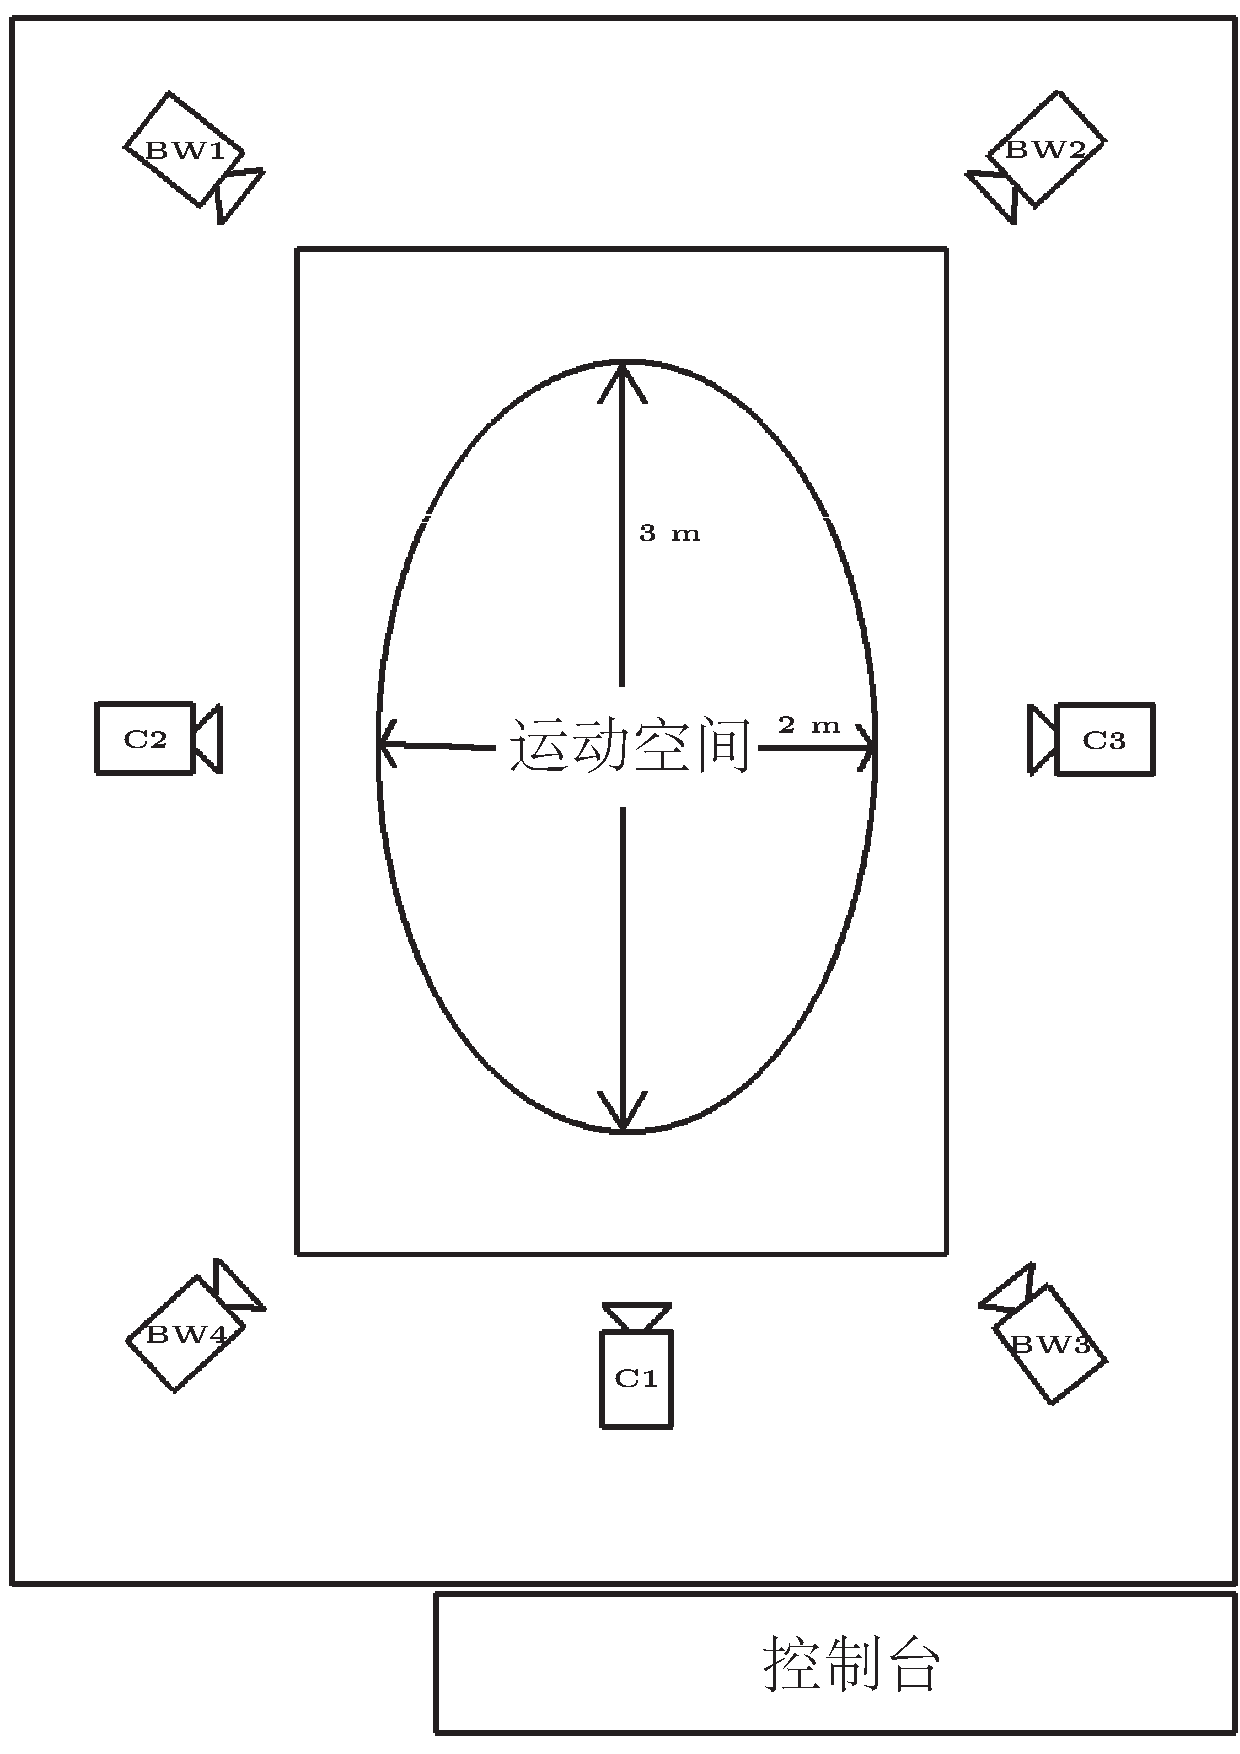
\includegraphics[height=8cm]{camera.pdf}\\
  \caption{相机摆放位置}\label{fig:camera}
\end{figure}

\begin{figure}[htbp]
  \centering
  \subcaptionbox{S1}{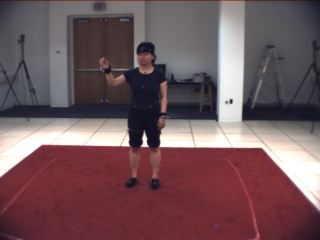
\includegraphics[width=0.4\textwidth]{S1}}\hspace{.5cm}
  \subcaptionbox{S2}{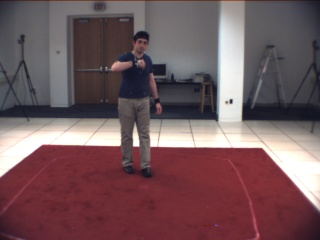
\includegraphics[width=0.4\textwidth]{S2}}\\
  \subcaptionbox{S3}{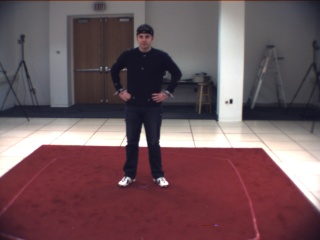
\includegraphics[width=0.4\textwidth]{S3}}\hspace{.5cm}
  \subcaptionbox{S4}{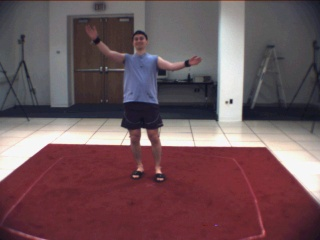
\includegraphics[width=0.4\textwidth]{S4}}
  \caption{HumanEva-I样例}\label{fig:demo}
\end{figure}

然而,数据库只对部分视频资料给出了运动姿态的ground-truth,四号演员的所有视频都只能用来测试,一到三号演员也有一半视频都没有ground-truth。此外,由于运动捕捉系统本身的问题,并不是对所有视频帧都能给出正确的三维姿态,因此经过筛选后\cite{Poppe2007}\cite{bo2010twin}文章所使用的训练数据如表\ref{tab:poppe}所示。在本文中,训练使用的帧数比\cite{Poppe2007}\cite{bo2010twin}文章较多,具体见表\ref{tab:mydataset}。导致两者训练数据不一致的原因可能是对有效帧的判断条件不一样,本文没有仔细追究。

\begin{table}[htbp]
  \centering
  \caption{\cite{Poppe2007}\cite{bo2010twin}文章所用帧数统计}
  \label{tab:poppe}
    \begin{tabular}{lcccc}
      \toprule[1.5pt]
      动作 & Subject1 & Subject2 & Subject3 & Total \\\midrule[1pt]
      走路 & 1176 & 876 & 895 & 2947 \\
      慢跑 & 439 & 795 & 831 & 2065 \\
      投掷 & 217 & 806 & 0 & 1023\\
      挥手 & 801 & 681 & 214 & 1696\\
      拳击 & 502 & 464 & 933 & 1889\\
      合计 & 3135 & 3622 & 2873 & 9630\\
      \bottomrule[1.5pt]
    \end{tabular}
\end{table}

\begin{table}[htbp]
  \centering
  \caption{本文所用帧数统计}
  \label{tab:mydataset}
    \begin{tabular}{lcccc}
      \toprule[1.5pt]
      动作 & Subject1 & Subject2 & Subject3 & Total \\\midrule[1pt]
      走路 & 1220 & 913 & 976 & 3109 \\
      慢跑 & 506 & 824 & 897 & 2227 \\
      投掷 & 217 & 815 & 0 & 1032\\
      挥手 & 872 & 690 & 260 & 1822\\
      拳击 & 576 & 470 & 996 & 2042\\
      合计 & 3391 & 3712 & 3129 & 10232\\
      \bottomrule[1.5pt]
    \end{tabular}
\end{table}



\section{人体三维骨架表示}
\label{sec:skeleton}

本文采用的人体三维骨架表示方法同\cite{bo2010twin},将人体用20个关节点来描述,每个关节点用$\mathbf{P}=(x,y,z)$三维坐标表示,串联起来构成$20\times3=60$维向量。在二维图像上表示骨架如图\ref{fig:2Ddemo},三维表示如图\ref{fig:3Ddemo},20个关节点的具体含义参见表\ref{tab:20}。为了使每个骨架对齐,我们把躯干远端作为三维坐标的原点,所有其他点坐标都根据原点做平移变换。

\begin{figure}[htbp]
  \centering
  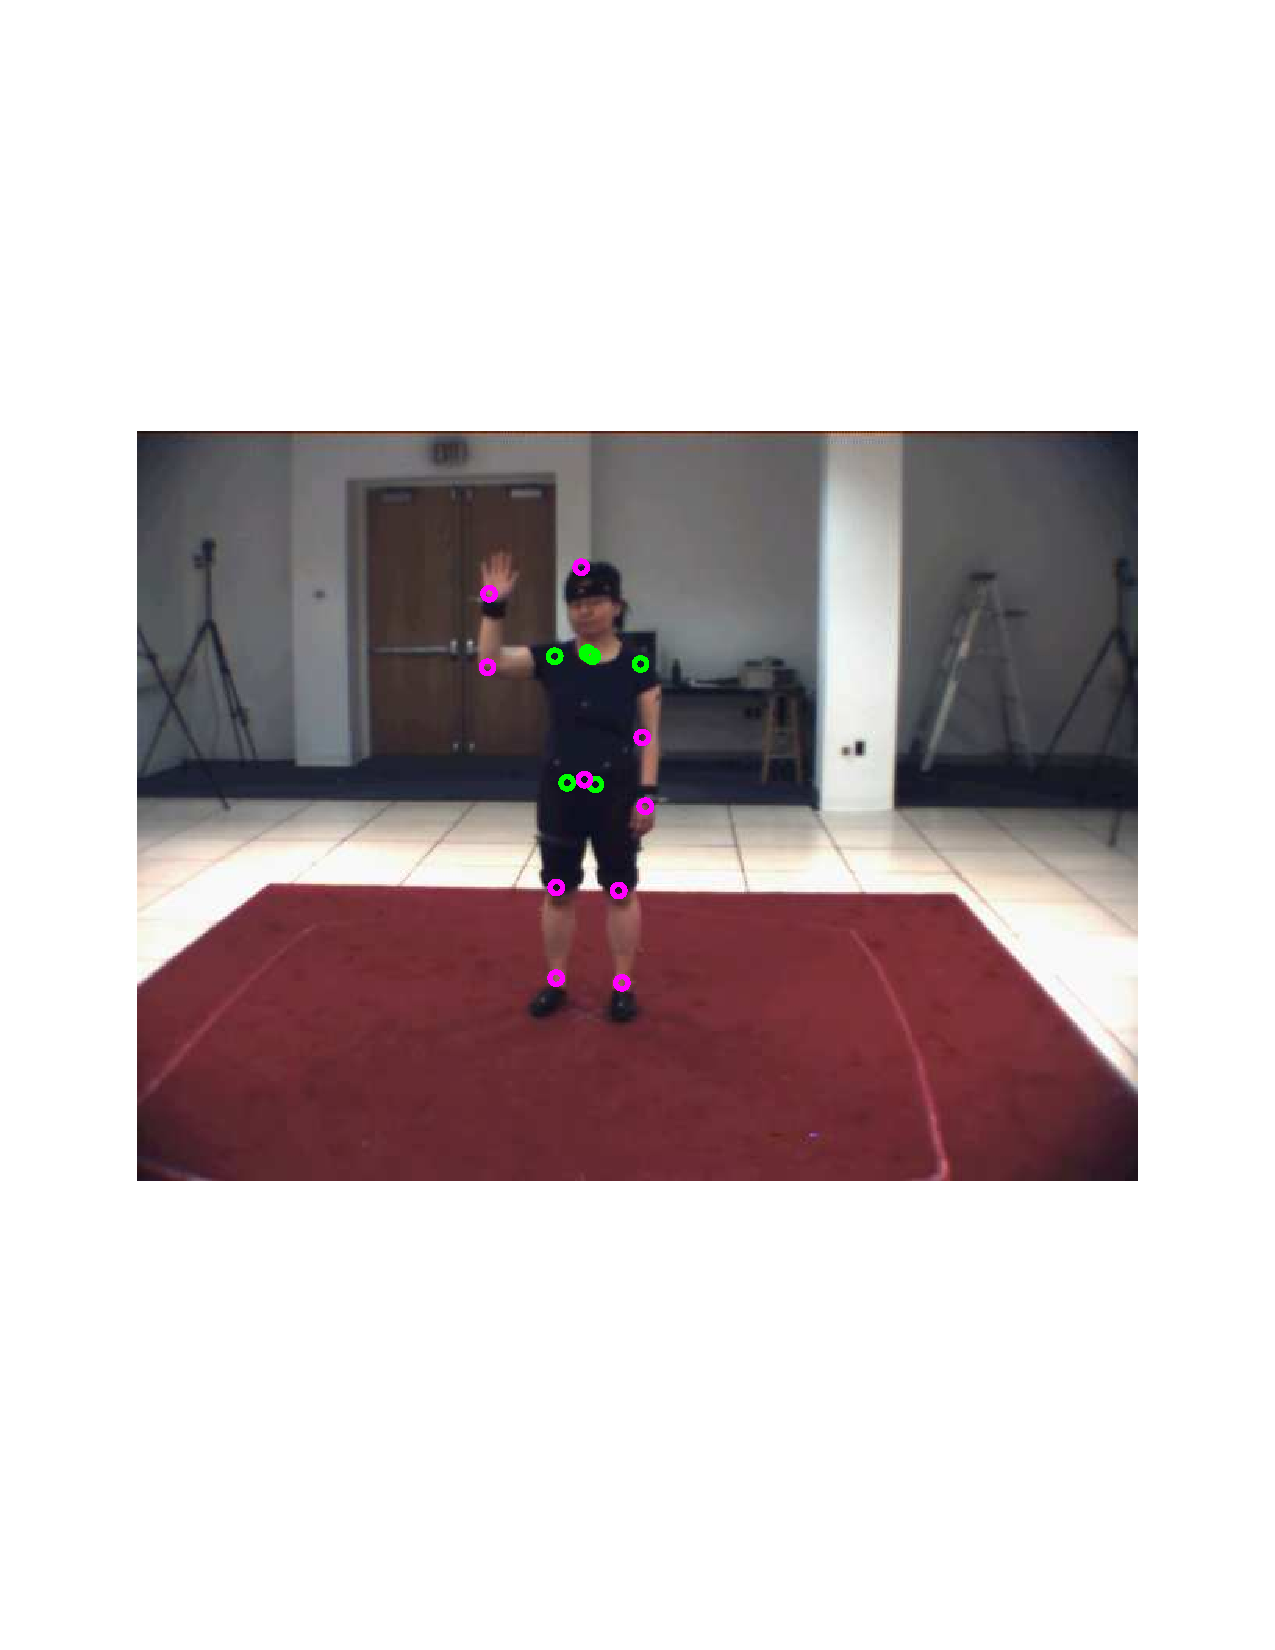
\includegraphics[width=0.7\textwidth]{2Dpose}\\
  \caption{二维骨架表示}\label{fig:2Ddemo}
\end{figure}

\begin{figure}[htbp]
  \centering
  \subcaptionbox{}{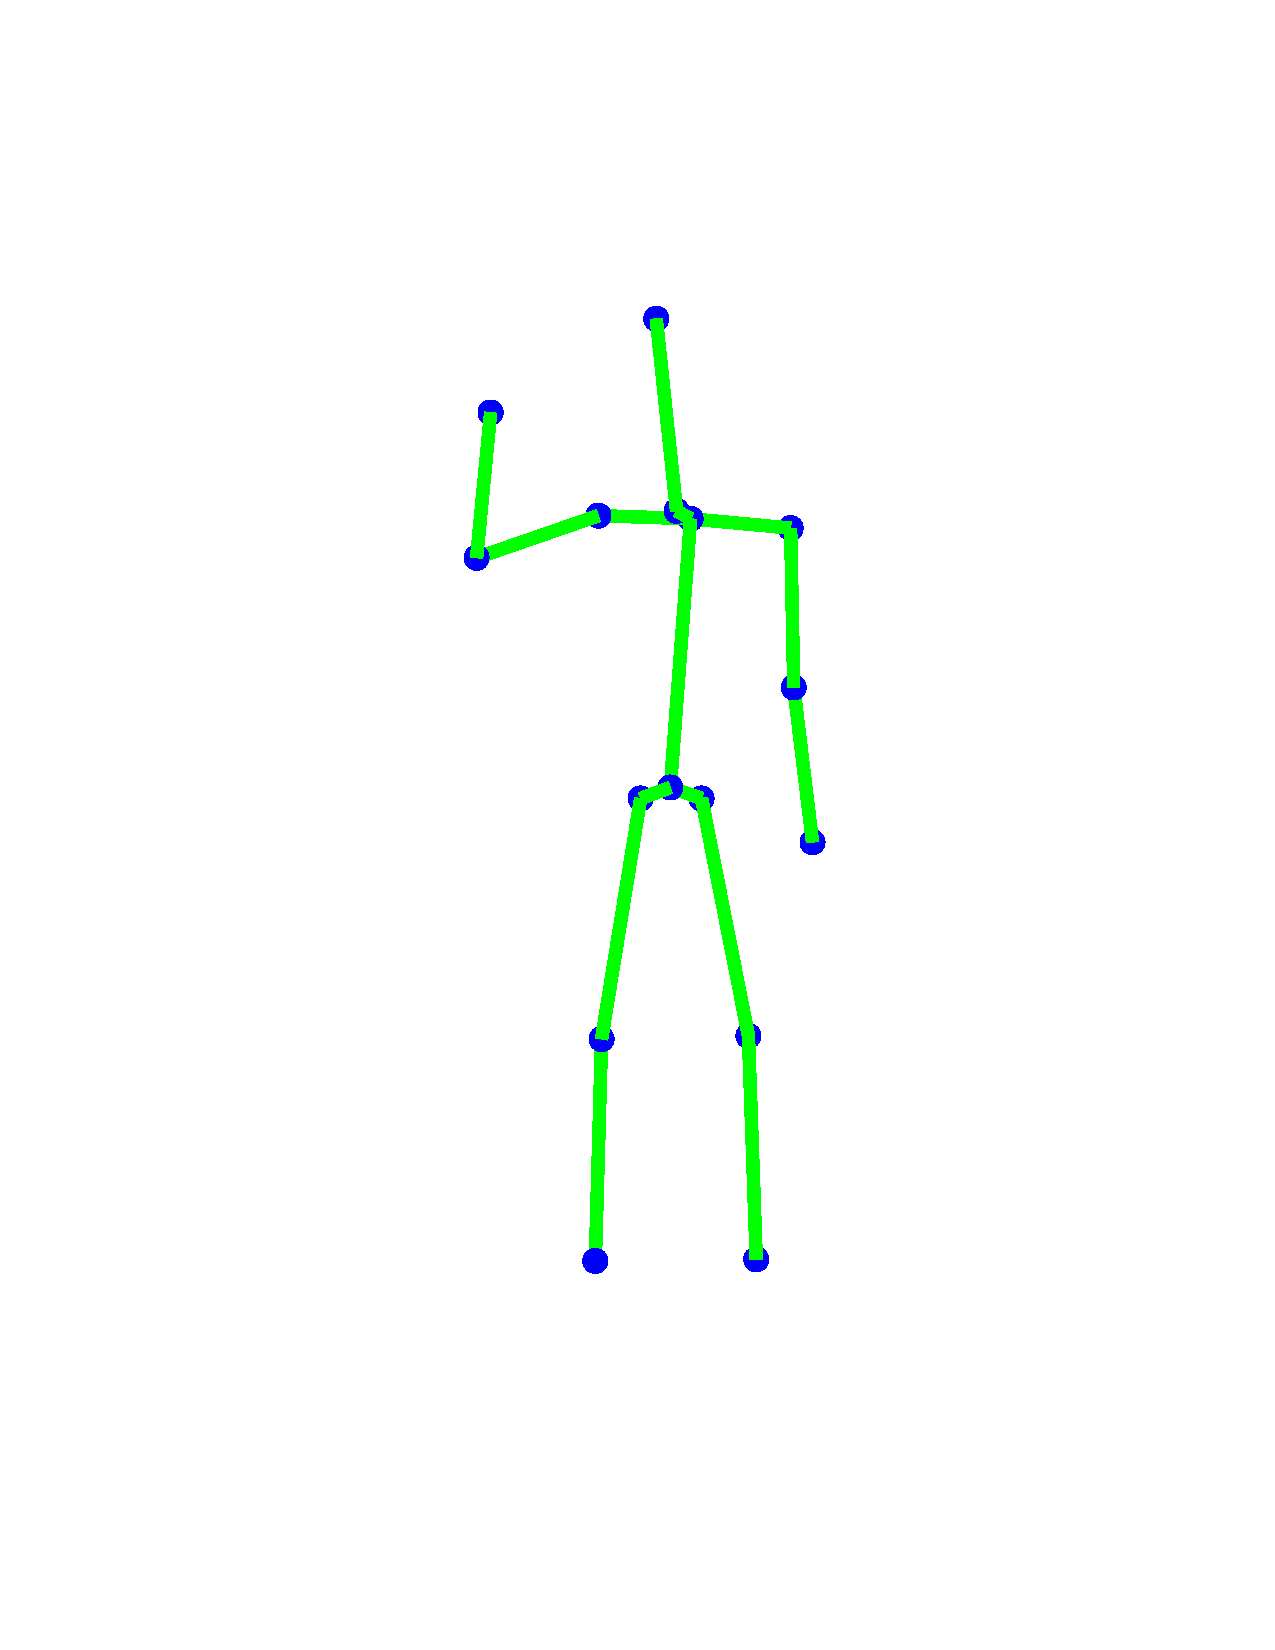
\includegraphics[height=6cm]{3D_1}}\hspace{1cm}
  \subcaptionbox{}{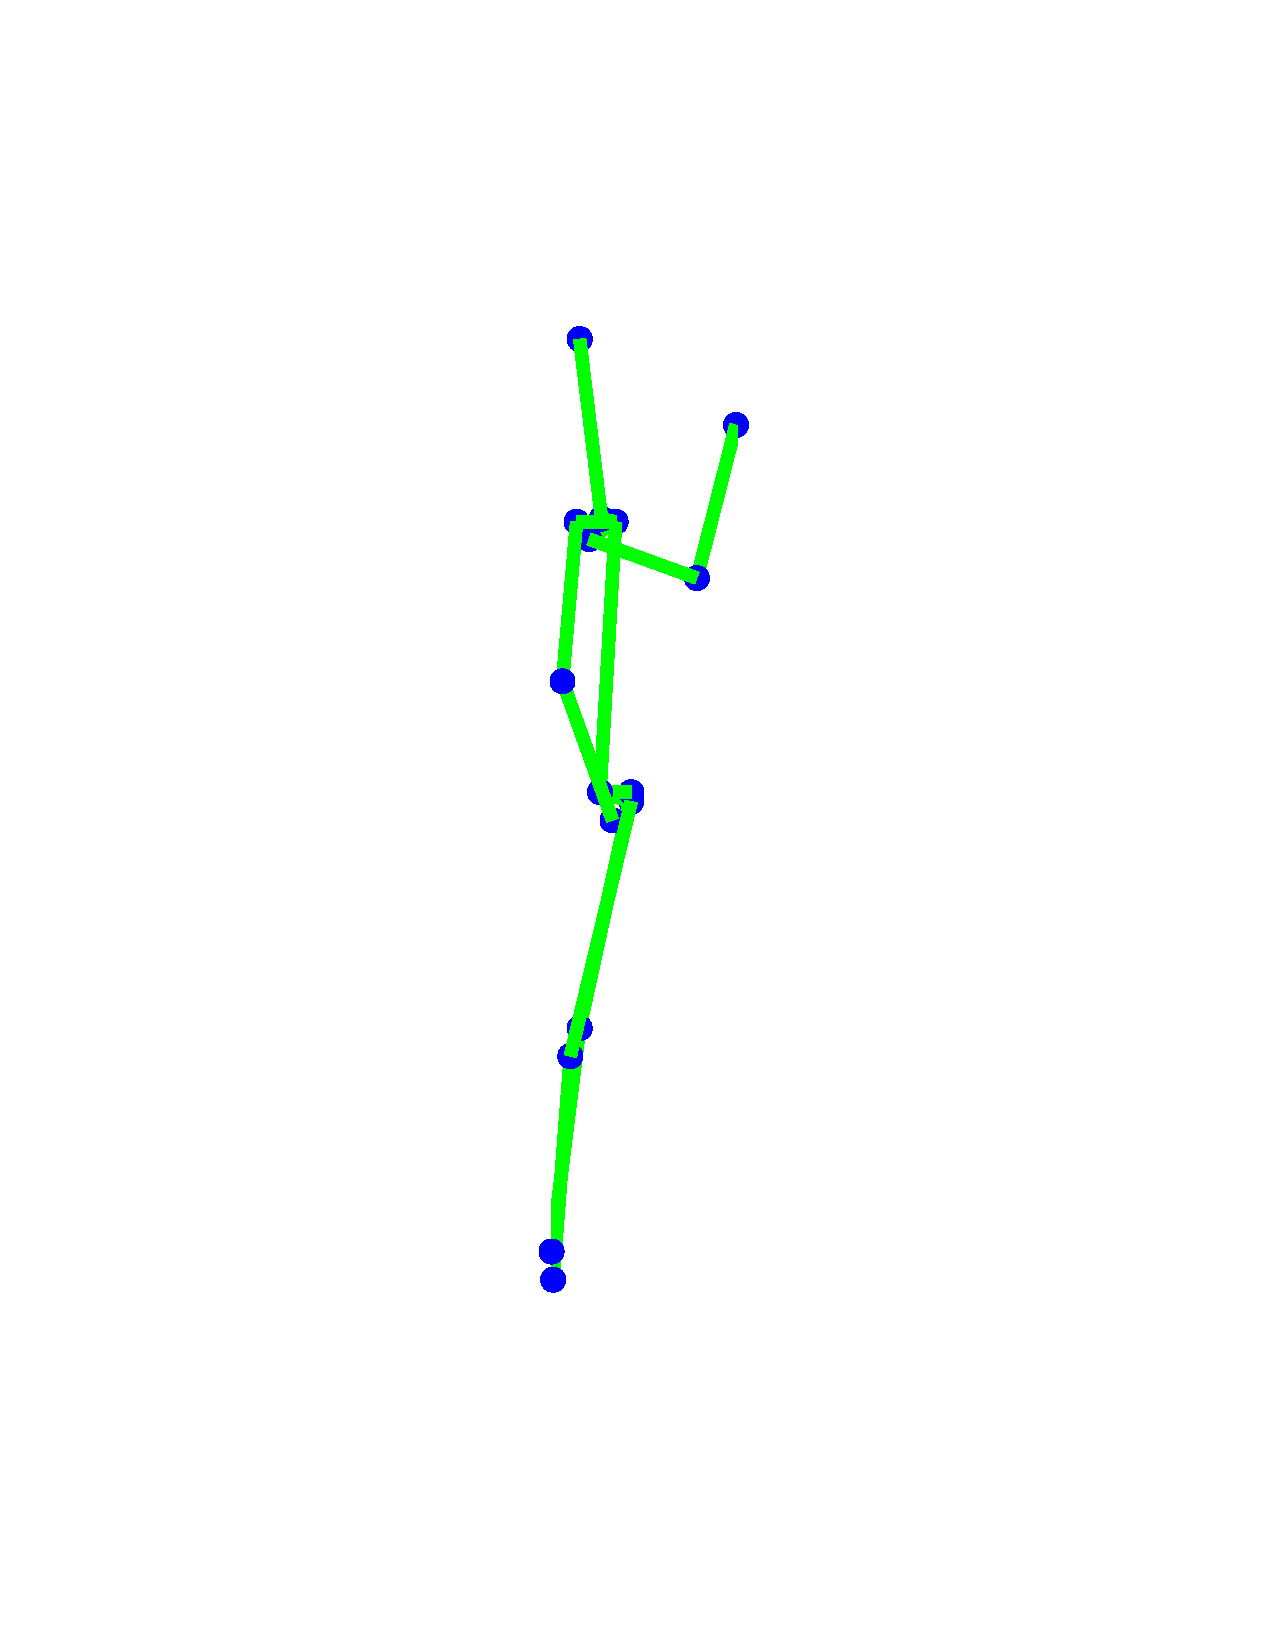
\includegraphics[height=6cm]{3D_2}}\hspace{1cm}
  \subcaptionbox{}{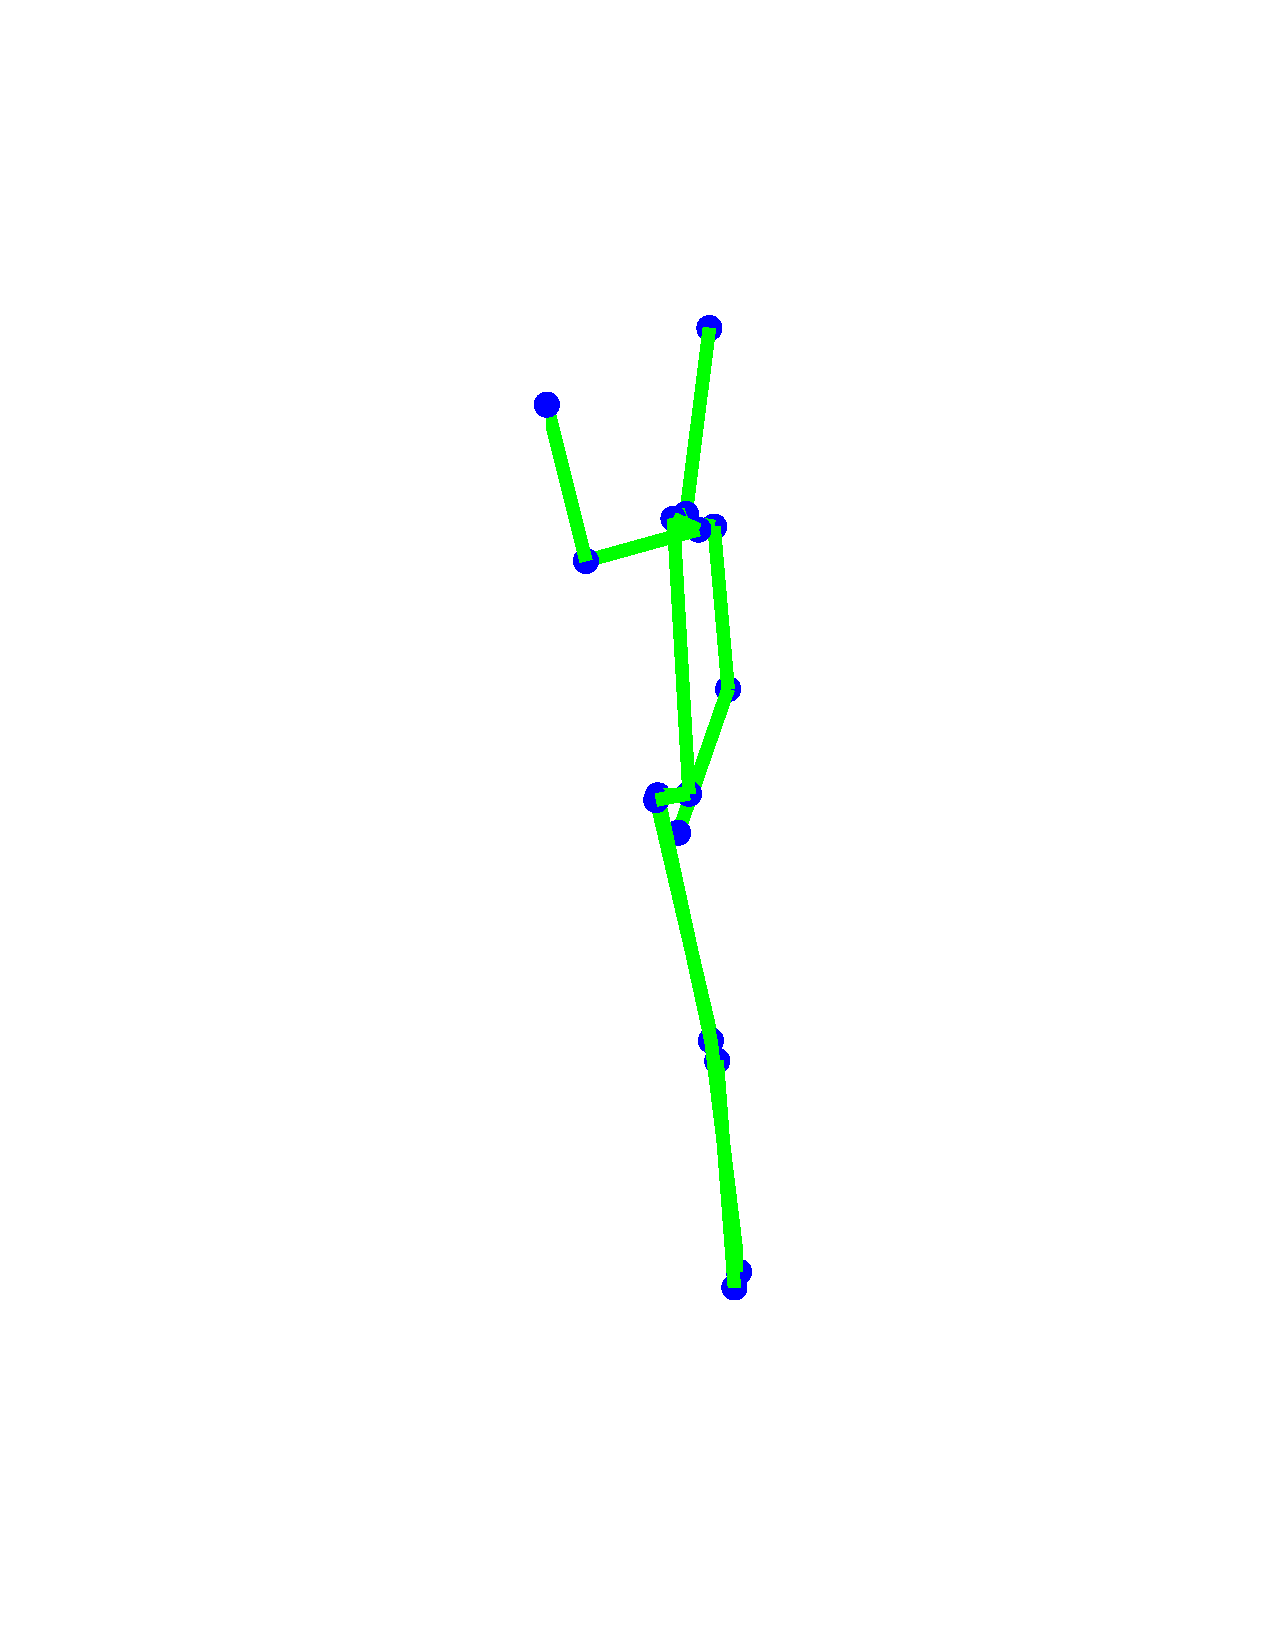
\includegraphics[height=6cm]{3D_3}}
  \caption{三维骨架表示}\label{fig:3Ddemo}
\end{figure}

\begin{table}[htbp]
  \centering
  \begin{tabular}{ccccccccccc}
  \toprule[1.5pt]
    & \multirow{2}{4em}{躯干}  & \multirow{2}{4em}{头部}  & \multicolumn{4}{c}{胳膊} & \multicolumn{4}{c}{腿}\\
    & & & 左前 & 左后 & 右前 & 右后 & 左前 & 左后 & 右前 & 右后 \\\midrule[1pt]
   近端 & 1 & 1 & 1 & 1 & 1 & 1 & 1 & 1 & 1 & 1 \\
   远端 & 1 & 1 & 1 & 1 & 1 & 1 & 1 & 1 & 1 & 1 \\
   \bottomrule[1.5pt]
  \end{tabular}
  \caption{关节点构成}\label{tab:20}
\end{table}
